\documentclass{beamer}
\usetheme{Warsaw}
\useinnertheme{circles}
\useoutertheme[subsection=false]{smoothbars}
\usepackage[utf8x]{inputenc}
\usepackage[czech]{babel}
\usepackage[T1]{fontenc}
\usepackage{listings}
\usepackage{tikz}
\lstset{basicstyle=\tiny\ttfamily}
\logo{
\includegraphics[height=0.5cm]{brmlab.pdf}}

\begin{document}

\AtBeginSection[]
{
  \begin{frame}
    \frametitle{Outline}
    \tableofcontents[currentsection]
  \end{frame}
}

\title{brmiversity: Umělá inteligence \\ a teoretická informatika}
\subtitle{Přednáška č. 4}
\author{Petr Baudiš $\langle${\tt pasky@ucw.cz}$\rangle$}
\institute{
	brmlab 2011\\
	\vskip 1ex
	\pgfdeclareimage[height=4ex]{ccbysa}{by-sa.pdf}
	\pgfuseimage{ccbysa}
}
\date{}
\frame{\titlepage}

\section{Neuronové sítě}

\subsection{}
\begin{frame}{Umělá neuronová síť}
\begin{itemize}
\item Umělé neurony (``výpočetní krabičky'') \\ dostávají vstupy (čísla) a na jejich \\ základě generují výstup (číslo)
\item Obvykle: Vrstvy striktně oddělené, \\ vstupní vrstva se vstupy zvnějšku, \\ výstupní vrstva s výstupem pro uživatele, \\ skryté vrstvy vyhodnocují různé charakteristiky vstupů
\item Dnes: Jediný umělý neuron
\end{itemize}
\begin{tikzpicture}[remember picture,overlay]
  \node [xshift=-4.5cm,yshift=-6cm,above right] at (current page.north east)
    {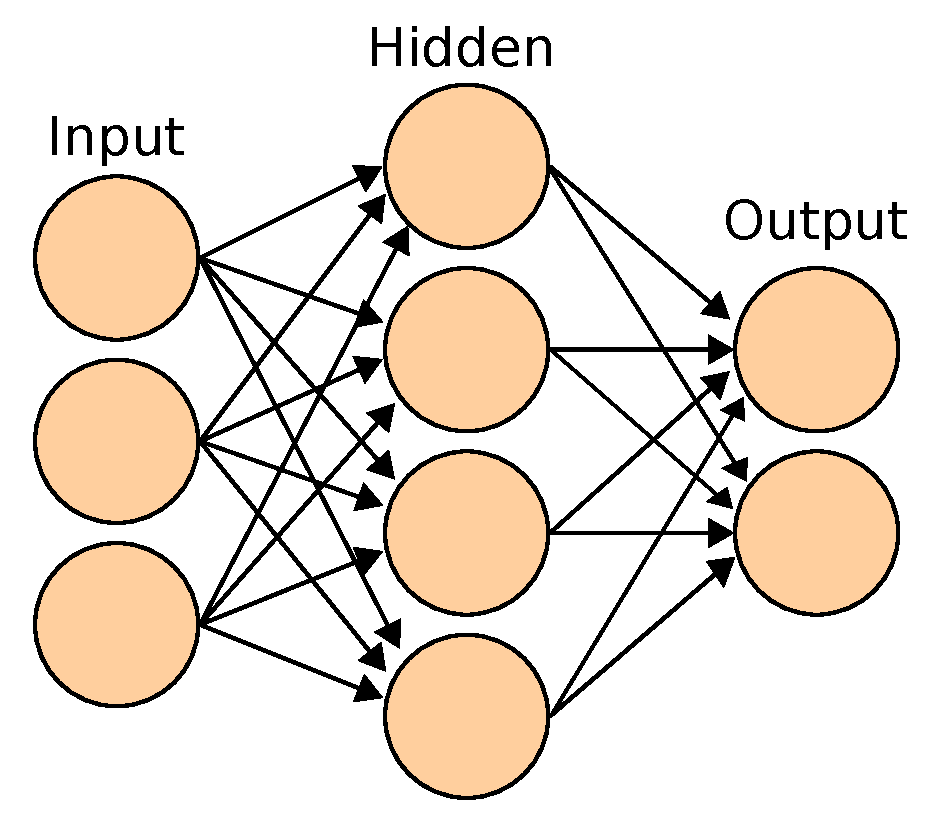
\includegraphics[width=4cm]{ANN.pdf}};
\end{tikzpicture}
\end{frame}

\subsection{}
\begin{frame}{Perceptron}
\begin{columns}
\begin{column}{4cm}
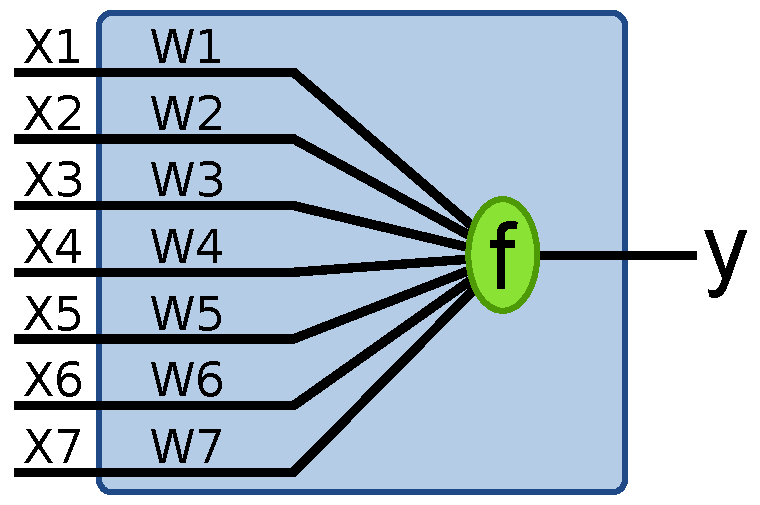
\includegraphics[width=4cm]{Perceptron.pdf}
\end{column}
\begin{column}{7cm}
\begin{itemize}
\item $n$ vstupů a práh $\Leftarrow$ výstup
\item Lineární kombinace --- vstupy mají různé váhy,\\ vynásobíme, sečteme a otestujeme
\item Výstup je 1/0 nebo něco složitějšího
\pause
\item Vstup $\vec x$, váhový vektor $\vec w$, práh $b$
\item $\sum_{i=0}^n w_i \cdot x_i > b$
\item Zjednodušení --- virtuální vstup pro práh
\end{itemize}
\end{column}
\end{columns}
\end{frame}

\subsection{}
\begin{frame}{Geometrická interpretace}
\begin{center}
\includegraphics[width=5cm]{perceptron_linear.png}
\includegraphics[width=5cm]{perceptron_update.png}
\end{center}
\end{frame}

\subsection{}
\begin{frame}{Co dokáže perceptron?}
\begin{columns}
\begin{column}{7cm}
\begin{itemize}
\item Lze vzorky čistě rozdělit podrovinou?
\item {\bf Lineární separabilita} množin
\item Omezení --- např. XOR potřebuje ``dvě čáry''
\end{itemize}
\end{column}
\begin{column}{4cm}
\includegraphics[width=4cm]{xor_solve.png}
\end{column}
\end{columns}
\end{frame}

\subsection{}
\begin{frame}{Učení perceptronu}
\begin{itemize}
\item ``Rotační'' algoritmus
\item Náhodná inicializace přímky
\item Iterujeme učení podle vstupních množin:
\begin{itemize}
\item Postupně iterujeme body a klasifikujeme
\item Správná klasifikace --- neděláme nic
\item Špatná klasifikace --- pootočíme vektor, aby ``pojmul'' i nový bod
\end{itemize}
\end{itemize}
\begin{tikzpicture}[remember picture,overlay]
  \node [xshift=-5cm,yshift=-5cm,above right] at (current page.north east)
    {\includegraphics[width=5cm]{perceptPict-2.png}};
\end{tikzpicture}
\end{frame}

\subsection{}
\begin{frame}{Učení perceptronu}
\begin{itemize}
\item Geometrické pozorování: $\vec w \cdot \vec x > 0$, \\ pak úhel mezi nimi je menší než $90 \deg$
\item Geometrické pozorování: Sečteme-li dva \\ vektory, vyjde nám vektor ``mezi''
\item Výstup je 0 a měl být 1: $w_i' = w_i + x_i(t)$
\item Výstup je 1 a měl být 0: $w_i' = w_i - x_i(t)$
\end{itemize}
\begin{tikzpicture}[remember picture,overlay]
  \node [xshift=-5cm,yshift=-5cm,above right] at (current page.north east)
    {\includegraphics[width=5cm]{perceptPict-2.png}};
\end{tikzpicture}
\end{frame}

\subsection{}
\begin{frame}{Otázky?}
\begin{center}
Příště: Vícevrstvé neuronové sítě a jejich učení (backpropagation).
\end{center}
\end{frame}

\section{Umělá inteligence}

\subsection{}
\begin{frame}{Filosofie}
\begin{itemize}
\item Silná vs. slabá AI
\item AI-complete úlohy
\item Bude víc 23.11.
\item Dnes jeden příklad slabé AI (je AI-complete?)
\end{itemize}
\end{frame}

\subsection{}
\begin{frame}{Matematické hry}
\begin{itemize}
\item Teorie her --- hráči se střídají v akcích, každý dostane nějakou výplatu po dokončení sekvence akcí
\item Hry dvou hráčů s úplnou informací a nulovým součtem
\end{itemize}
\end{frame}

\subsection{}
\begin{frame}{Minimaxový strom}
\begin{itemize}
\item ``Adversarial planning''
\item Tah je tak dobrý jako nejnepříjemnější tah protihráče
\item Omezení na hloubku stromu --- vyhodnocovací funkce
\end{itemize}
\begin{center}
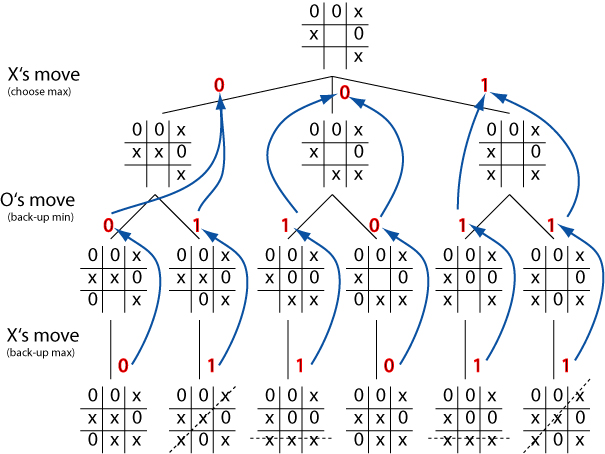
\includegraphics[width=7cm]{minimax-illustration.jpg}
\end{center}
\end{frame}

\subsection{}
\begin{frame}{$\alpha,\beta$ prořezávání}
\begin{itemize}
\item Základní urychlovací heuristika
\item Pamatujeme si nejhorší a nejlepší hodnoty z minimaxových sousedů, zařízneme prohledávání uzlu, je-li jasné, že bude horší (max, $\alpha$) nebo lepší (min, $\beta$)
\item Pro efektivitu je důležité pořadí vyhodnocování tahů
\end{itemize}
\begin{center}
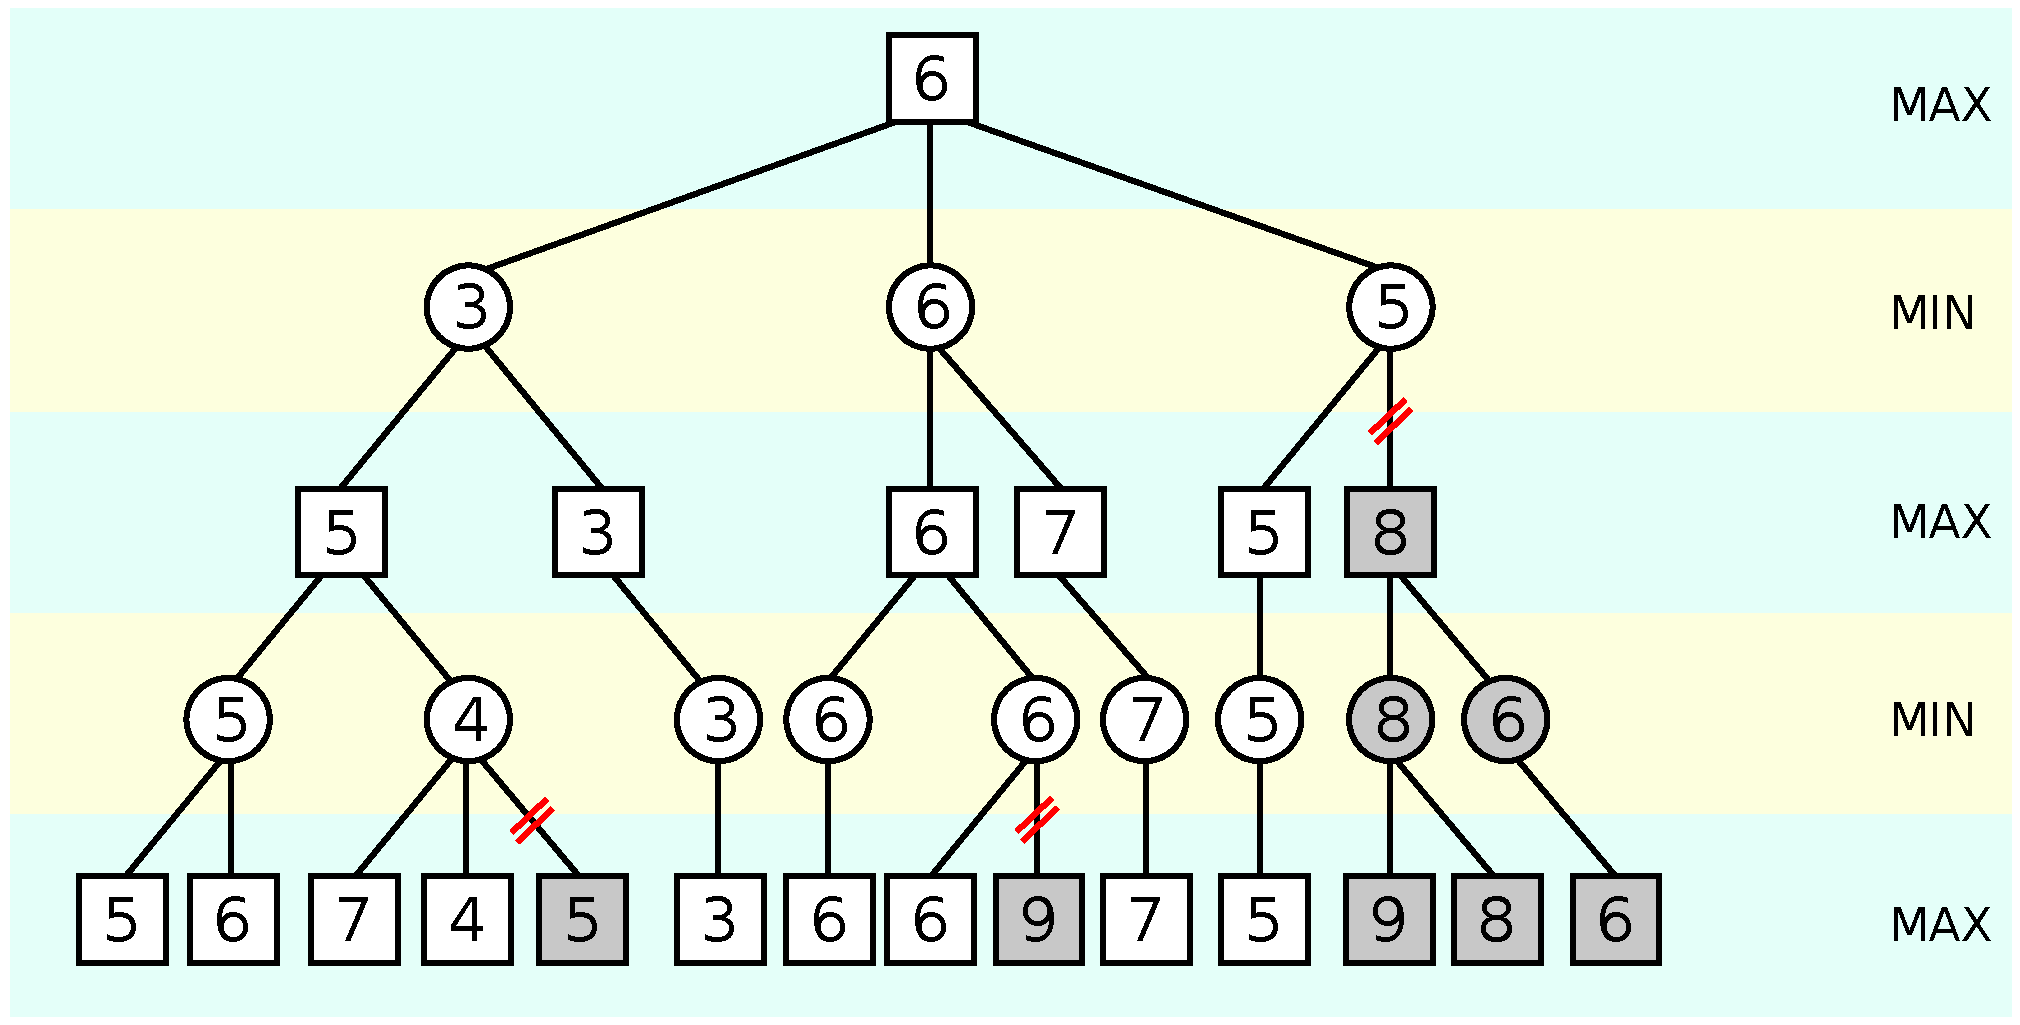
\includegraphics[width=6cm]{AB_pruning.pdf}
\end{center}
\end{frame}

\subsection{}
\begin{frame}{Další vylepšení}
\begin{itemize}
\item Transpoziční tabulky
\item Prořezávání, singular extensions, atd.
\item Problémy --- dobrá funkce, větvící faktor, efekt horizontu
\end{itemize}
\end{frame}

\subsection{}
\begin{frame}{Monte Carlo Tree Search}
\begin{itemize}
\item Technika Monte Carlo
\item Minimaxový strom s očekáváními
\item Multi-armed bandit
\end{itemize}
\begin{center}
\includegraphics[width=8cm]{mcts.png}
\end{center}
\end{frame}

\subsection{}
\begin{frame}{Otázky?}
\begin{center}
Příště: Prohledávání v grafech.
\end{center}
\end{frame}

\section{Základní algoritmy}

\subsection{}
\begin{frame}{Levenšteinova editační vzdálenost}
\begin{itemize}
\item Dva stringy; editace jsou přidání, změna, odebrání
\item Dynamický algoritmus:
\end{itemize}

\begin{center}
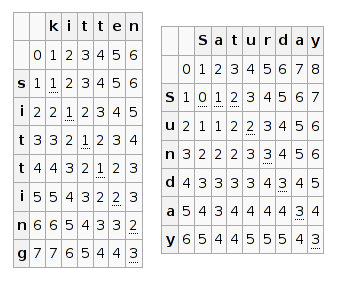
\includegraphics[width=6cm]{levehnstein.png}
\end{center}
\end{frame}

\subsection{}
\begin{frame}{Další způsoby porovnávání}
\begin{itemize}
\item Myersův algoritmus (nejdelší společná podposloupnost \\ neboli editační skript; jen $+$ a $-$)
\item bdiff (nejdelší společný podřetězec --- rekurzivně)
\item xdelta (rsync; Rabinovo hashování)
\end{itemize}
\end{frame}

\section{Složitost}

\subsection{}
\begin{frame}{Metody tvorby algoritmů}
\begin{itemize}
\item Kuchařka pro efektivní algoritmy na obecné třídy problémů
\item Rozděl a panuj --- problém rozdělíme na podproblémy \\ a ty počítáme rekurzivně
\item Hladový algoritmus --- problém budujeme inkrementálně, v~každé chvíli víme, kudy dál
\item Dynamický algoritmus --- problém budujeme inkrementálně, sdílíme výsledky jednodušších podproblémů
\end{itemize}
\end{frame}

\subsection{}
\begin{frame}{Rozděl a panuj --- příklad}
\begin{itemize}
\item Binární vyhledávání: \\
	\only<1>{1 3 9 10 12 13 17 19 24 26 27 30 31}
	\only<2>{1 3 9 10 12 13 {\bf 17} 19 24 26 27 30 31}
	\only<3>{1 3 9 10 12 13 {\tiny 17 19 24 26 27 30 31}}
	\only<4>{1 3 {\bf 9} 10 12 13 {\tiny 17 19 24 26 27 30 31}}
	\only<5>{{\tiny 1 3 9} 10 12 13 {\tiny 17 19 24 26 27 30 31}}
	\only<6>{{\tiny 1 3 9} 10 {\bf 12} 13 {\tiny 17 19 24 26 27 30 31}}
	\only<7>{{\tiny 1 3 9} 10 {\tiny 12 13 \tiny 17 19 24 26 27 30 31}}
\item Quicksort
\item Asymptotická složitost --- Master Theorem \\ (matematika viz Wikipedie)
\end{itemize}
\end{frame}

\subsection{}
\begin{frame}{Hladový algoritmus --- příklad}
\begin{itemize}
\item Minimální kostra (připomenutí)
\item Rozvrhovací problém
\item Dijkstra
\pause
\vskip 3ex
\item Hladový algoritmus lze použít, pokud problém vykazuje {\em optimální podstrukturu}
\item Matematická abstrakce --- {\bf matroid} $M = (E,I)$, \\ $E$ je základní množina, $I$ je systém nezávislých podmnožin:
\begin{itemize}
\item $\emptyset \in I$ (prázdná množina je nezávislá)
\item $A \in I, A' \subset A \quad\Rightarrow\quad A' \in I \quad \forall A, A'$ (dědičnost)
\item $A \in I \land B \in I \land |A| > |B| \quad\Rightarrow\quad \exists\, x \in A, \quad B \cup {x} \in I$
\end{itemize}
\end{itemize}
\end{frame}

\subsection{}
\begin{frame}{Dynamický algoritmus}
\begin{itemize}
\item Editační vzdálenost
\item Fibonacciho posloupnost
\item Dijkstra
\vskip 3ex
\item Optimální podstruktura a překrývající se podproblémy
\end{itemize}
\end{frame}

\subsection{}
\begin{frame}{Třídění}
\begin{itemize}
\item Jak dlouho trvá třídění? Spodní odhad je $O(n\cdot\log n)$
\item Vyhledávací strom modeluje rozhodovací strom algoritmu
\item Nebo ano? Radix sort, ale je to podvod!
\end{itemize}
\begin{center}
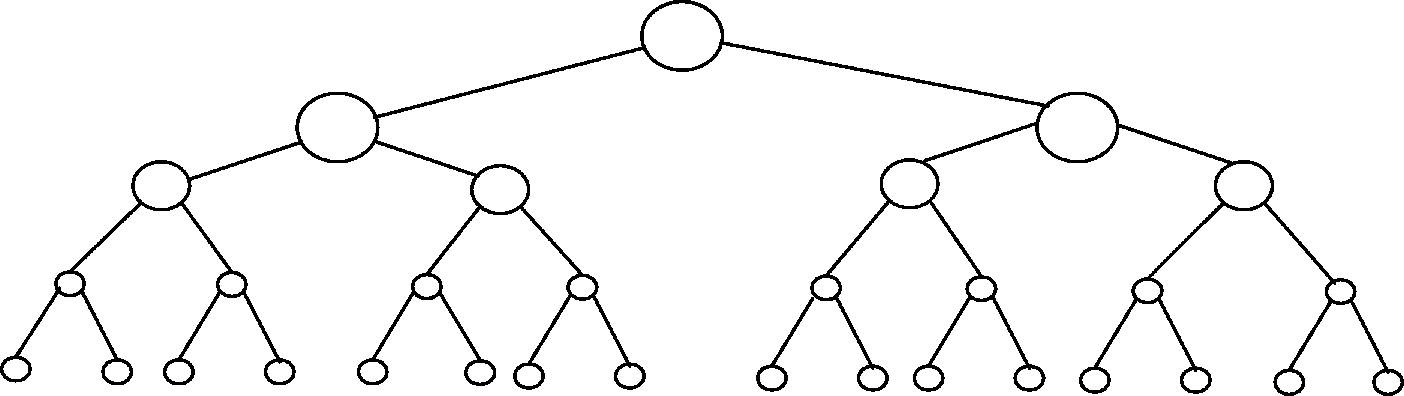
\includegraphics[width=8cm]{fullbintree.png}
\end{center}
\end{frame}

\subsection{}
\begin{frame}{Otázky?}
\begin{center}
Příště: Pravděpodobnostní algoritmy.
\end{center}
\end{frame}

\section{Vyčíslitelnost}

\subsection{}
\begin{frame}{Rekapitulace}
\begin{itemize}
\item Rekapitulace: Nezajímá nás, jak rychle to poběží, \\ ale jestli to někdy doběhne.
\item Zkoumáme výpočetní {\em možnosti} algoritmů.
\vskip 3ex
\item Minule jsme přemýšleli, čím vším lze algoritmy vykonávat \\ (a že je to ekvivalentní).
\item Zapomněli jsme (mj.) na {\bf celulární automaty}! % TODO: obrazek
\end{itemize}
\end{frame}

\subsection{}
\begin{frame}{Halting Problem}
\begin{itemize}
\item Máme program $z=x(y)$; $x, y, z$ jsou čísla \\ (kód, parametr / vstup, návratová hodnota / výstup)
\item Program doběhne (v konečném čase) a vrátí hodnotu \\ ({\em řeší} problém), nebo se zacyklí
\pause
\vskip 3ex
\item Nekonečná smyčka v závislosti na datech, \\ schovaná uprostřed složitého kódu
\item Halting Problem: Zacyklí se program $x$ na vstupu $y$?
\item Dokážeme napsat program, který řeší halting problem?
\end{itemize}
\end{frame}

\subsection{}
\begin{frame}{Halting Problem: Důkaz}
\begin{itemize}
\item Důkaz sporem --- dejme tomu, že máme funkci $HALT(x,y)$, $x$ je kód programu ($c(FUNKCE)$) a $y$ je vstup
\item Ukážeme, že existence takové funkce způsobuje \\ logické trhliny v časoprostoru
\pause
\item Trik: Nadefinujme si funkci $PODRAZ(x) \downarrow \quad \Longleftrightarrow \quad HALT(x,x)=NE$
\begin{itemize}
\item Tedy $PODRAZ(x)$ zavolá funkci $HALT(x,x)$
\item Pokud by se program $x$ na vstupu $x$ (kód sama sebe) zastavil, $PODRAZ(x)$ se zacyklí
\item Pokud by se program $x$ na vstupu $x$ (kód sama sebe) zacyklil, $PODRAZ(x)$ doběhne
\end{itemize}
\pause
\item Zavolejme $PODRAZ(c(PODRAZ))$!
\item $HALT(c(PODRAZ),c(PODRAZ)) = ANO \quad \Longleftrightarrow \quad PODRAZ(c(PODRAZ)) \downarrow \quad \Longleftrightarrow \quad HALT(c(PODRAZ),c(PODRAZ)) = NE$
\item To je spor, $ANO \ne NE$.
\end{itemize}
\end{frame}

\subsection{}
\begin{frame}{Otázky?}
\begin{center}
Příště: Rekurzivní a rekurzivně spočetné množiny.
\end{center}
\end{frame}

\subsection{}
\begin{frame}{Děkuji vám}
\begin{center}
{\bf pasky@ucw.cz}

\vskip 6ex

Příště: {\bf Nebude.}

\vskip 6ex

Popříště: Prohledávání grafů a hledání cesty (základní algoritmy, umělá inteligence, adaptivní agenti), neuronové sítě, vyčíslitelnost.
\end{center}
\end{frame}

\end{document}
